\subsection{Benchmarking Against Published LDL Feature Selection Scoring Cores}
\label{sec:paper-published}

To evaluate competitive standing against state-of-the-art methodology, we benchmark the proposed framework against the scoring cores of three representative Label Distribution Learning (LDL) feature selection algorithms:
\begin{enumerate}[label=(\arabic*), leftmargin=*]
	\item \textbf{GBFRS~\cite{Qian2023GBLDL}:} Granular-ball fuzzy rough dependency. To establish a rigorous baseline, fuzzy rough dependency $\gamma(P) = \frac{1}{n}\sum_{i}\sum_{k}\ell_i^k (R \!\downarrow\! D_k)(x_i)$ is computed directly using Gaussian similarities with exact lower approximations, evaluated under matched-cardinality (GBFRS-$k$) and cost-effective greedy selection (GBFRS-Budget).
	\item \textbf{DSIM~\cite{DL}:} Dual-similarity metric maximizing the normalized Hilbert-Schmidt covariance between feature-space and label-distribution affinity matrices, evaluated under matched-$k$ (DSIM-$k$) and matched-budget (DSIM-Budget) settings.
	\item \textbf{FSLC~\cite{QX}:} Feature similarity and label correlation ranking incorporating an MIFS-style feature-redundancy penalty.
\end{enumerate}
All scoring cores are integrated under identical cross-validation folds, feature scalings, and cost assignments across sixty independent splits spanning four benchmark datasets: \textit{Natural Scene}, \textit{SBU-3DFE}, \textit{Yeast-cold}, and \textit{Human Gene} (17,892 instances, 36 attributes, 68 continuous labels, serving as a high-dimensional label stress test). Section~\ref{par:published-expansion} extends the same protocol to the twenty-three datasets of the multi-domain expansion and to two additional recent scoring cores.

\begin{table}[htbp]
	\centering\small\renewcommand{\arraystretch}{1.25}\setlength{\tabcolsep}{5pt}
	\caption{Quantitative performance comparison against published LDL scoring cores at training size $n=576$ (mean across independent runs). Baselines marked with $k$ share feature cardinality with $G$; budget variants share $G$'s total acquisition cost $C(P)$.}
	\label{tab:published-main}
	\begin{tabular}{l l rrr}\hline
		Dataset & Selection Method & $k$ & Cost $C(P)$ & Test Brier $\pm$ SD\\\hline
		\textit{Natural Scene} & \textbf{$G$ (Proposed)} & \textbf{12.6} & \textbf{17.4} & \textbf{0.2511 $\pm$ 0.0176}\\
		& GBFRS-$k$~\cite{Qian2023GBLDL} & 12.6 & 70.0 & 0.2577 $\pm$ 0.0204\\
		& GBFRS-Budget & 4.6 & 17.4 & 0.2939 $\pm$ 0.0420\\
		& DSIM-$k$~\cite{DL} & 12.6 & 69.4 & 0.2687 $\pm$ 0.0142\\
		& DSIM-Budget & 14.2 & 17.4 & 0.2512 $\pm$ 0.0204\\\hline
		\textit{SBU-3DFE} & \textbf{$G$ (Proposed)} & \textbf{8.4} & \textbf{11.0} & \textbf{0.0315 $\pm$ 0.0013}\\
		& GBFRS-$k$ & 8.4 & 52.2 & 0.0309 $\pm$ 0.0010\\
		& GBFRS-Budget & 3.4 & 11.0 & 0.0323 $\pm$ 0.0027\\
		& DSIM-$k$ & 8.4 & 46.2 & 0.0316 $\pm$ 0.0013\\
		& DSIM-Budget & 10.2 & 11.0 & 0.0316 $\pm$ 0.0016\\\hline
		\textit{Yeast-cold} & \textbf{$G$ (Proposed)} & \textbf{2.6} & \textbf{7.2} & \textbf{0.0075 $\pm$ 0.0009}\\
		& GBFRS-$k$ & 2.6 & 13.0 & 0.0075 $\pm$ 0.0005\\
		& GBFRS-Budget & 2.4 & 7.0 & 0.0075 $\pm$ 0.0005\\
		& DSIM-$k$ & 2.6 & 13.2 & 0.0074 $\pm$ 0.0006\\
		& DSIM-Budget & 2.6 & 7.0 & 0.0075 $\pm$ 0.0005\\\hline
		\textit{Human Gene} & \textbf{$G$ (Proposed)} & \textbf{3.8} & \textbf{11.6} & \textbf{0.0187 $\pm$ 0.0046}\\
		& GBFRS-$k$ & 3.8 & 26.4 & 0.0188 $\pm$ 0.0046\\
		& GBFRS-Budget & 2.6 & 11.6 & 0.0187 $\pm$ 0.0046\\
		& DSIM-$k$ & 3.8 & 27.0 & 0.0184 $\pm$ 0.0044\\
		& DSIM-Budget & 4.4 & 11.6 & 0.0186 $\pm$ 0.0045\\
		\hline\end{tabular}
\end{table}

\begin{table}[htbp]
	\centering\small\renewcommand{\arraystretch}{1.25}\setlength{\tabcolsep}{4pt}
	\caption{Paired test Brier differences ($\Delta = \text{Brier}_G - \text{Brier}_{\text{Baseline}}$, negative values favor $G$) and head-to-head win counts across all 15 splits per dataset (60 independent splits pooled).}
	\label{tab:published-paired}
	\begin{tabular}{l rr rr rr rr}\hline
		& \multicolumn{2}{c}{\textit{Natural Scene}} & \multicolumn{2}{c}{\textit{SBU-3DFE}} & \multicolumn{2}{c}{\textit{Yeast-cold}} & \multicolumn{2}{c}{\textit{Human Gene}}\\
		\cline{2-3}\cline{4-5}\cline{6-7}\cline{8-9}
		Baseline Method & $\Delta$ & Wins & $\Delta$ & Wins & $\Delta$ & Wins\\\hline
		GBFRS-$k$ & $-0.0093$ & 8/15 & $+0.0002$ & 8/15 & $+0.0001$ & 9/15 & $-0.0000$ & 9/15\\
		GBFRS-Budget & $-0.0374$ & 13/15 & $-0.0021$ & 3/15 & $-0.0000$ & 5/15 & $-0.0001$ & 7/15\\
		DSIM-$k$ & $-0.0144$ & 12/15 & $-0.0003$ & 7/15 & $+0.0001$ & 8/15 & $+0.0002$ & 2/15\\
		DSIM-Budget & $-0.0014$ & 8/15 & $+0.0001$ & 8/15 & $-0.0000$ & 5/15 & $+0.0000$ & 4/15\\
		\hline\end{tabular}
\end{table}

\paragraph{Statistical Significance Analysis}
Pooling all 60 splits across the four benchmarks, a non-parametric Friedman test decisively rejects the null hypothesis of equivalent performance across methods ($\chi^2 = 25.06$, $p < 0.0001$). Post-hoc pairwise Wilcoxon signed-rank tests with Holm correction confirm that GBFRS-Budget is statistically significantly inferior to $G$ ($p_{\mathrm{Holm}} = 0.0004$). Meanwhile, $G$ achieves equivalent or superior predictive accuracy compared to GBFRS-$k$, DSIM-$k$, and DSIM-Budget ($p_{\mathrm{Holm}} \ge 0.44$) while consuming substantially lower acquisition expenditures.

\paragraph{Key Comparative Findings}
Tables~\ref{tab:published-main} and \ref{tab:published-paired} elucidate three fundamental strengths of our framework:
\begin{enumerate}[label=(\arabic*), leftmargin=*]
	\item \textbf{Significant Acquisition Cost Advantage:} On the higher-dimensional benchmarks (\textit{Natural Scene} and \textit{SBU-3DFE}), published cardinality-matched selectors (GBFRS-$k$ and DSIM-$k$) incur \textbf{four to five times higher acquisition costs} (e.g., $70.0$ and $69.4$ vs. $17.4$ on \textit{Natural Scene}; $52.2$ and $46.2$ vs. $11.0$ on \textit{SBU-3DFE}) while obtaining statistically indistinguishable or inferior Brier losses. Our framework strictly dominates these baselines on the cost--loss Pareto frontier.
	\item \textbf{Superiority of Internal Feasibility Guarding:} When constrained to the exact budget spent by $G$, pure dependency-based selection (GBFRS-Budget) degrades sharply on \textit{Natural Scene}, suffering higher Brier loss in 13 out of 15 splits ($+0.043$ mean excess loss). This empirical failure illustrates the divergence between heuristic representation scores and actual generalization loss, confirming the necessity of our inner validation loss guard ($L_{\max}$).
	\item \textbf{Adaptive Response to Near-Degenerate Label Regimes:} On \textit{Yeast-cold} and \textit{Human Gene}, all methods exhibit closely clustered Brier losses within $0.0002$. On these datasets, the uninformative global mean distribution baseline achieves optimal Brier scores ($0.0158$ on \textit{Human Gene} vs. $0.0181$--$0.0188$ for non-empty subsets). Our framework reliably detects this near-degenerate regime via internal validation, ensuring that cost-intensive attributes are not needlessly acquired when structural distribution signals are weak.
\end{enumerate}
\paragraph{Expansion Coverage and Recent Scoring Cores}
\label{par:published-expansion}
The matched-$k$ and matched-budget protocol was additionally executed on all twenty-three expansion datasets (three repeats each, sixty-nine dataset--repeat units), with $k$ and the budget matched to the frozen $G+$ selections and all evaluation moved to the reserved audit partition. Beyond the three original cores, we implemented two recent scoring cores under the identical unified protocol: \textbf{NRS}~\cite{Wu2025NRS}, a neighborhood rough set dependency for LDL ($\delta$-neighborhood lower approximations of the label-wise decision classes with $\delta = 0.1$ on min-max-normalized attributes, forward greedy on the dependency), and \textbf{FMI}~\cite{You2024FMI}, a fuzzy mutual information core (three-triangular-set fuzzification of attributes and label dimensions, MIFS-style redundancy penalty), following the neighborhood-rough-set and fuzzy-MI LDL selectors of 2025 and 2024 respectively. On the twenty datasets where the internal guard certifies the empty set, the matched protocols are degenerate ($k=0$, $C=0$): every scoring core, including NRS and FMI, returns the empty set and all methods tie exactly, confirming that no published core extracts transferable local signal from these domains under the same predictor either. Table~\ref{tab:expansion-published} therefore reports the informative subset (\textit{SJAFFE}, \textit{fbp5500}, \textit{RAF-ML}) in full.

\begin{table}[htbp]
\centering\small\renewcommand{\arraystretch}{1.25}\setlength{\tabcolsep}{4pt}
\caption{Published scoring cores on the informative expansion datasets (three-repeat means, reserved-audit Brier). Baselines marked $k$ share cardinality with $G+$; budget variants share its cost. On the twenty guard-empty datasets every matched protocol returns the empty set and ties exactly, so those units enter only the pooled statistics reported in the text.}
\label{tab:expansion-published}
\begin{tabular}{llrrr}\hline
Dataset & Method & Attributes & Cost & Audit Brier\\\hline
SJAFFE & \textbf{$G+$ (proposed)} & 10.0 & 28.3 & 0.0247\\
 & GBFRS k & 10.0 & 45.3 & 0.0263\\
 & GBFRS budget & 6.7 & 28.3 & 0.0264\\
 & DSIM k & 10.0 & 41.0 & 0.0247\\
 & DSIM budget & 18.3 & 28.3 & 0.0222\\
 & FSLC k & 10.0 & 40.0 & 0.0246\\
 & FSLC budget & 16.7 & 28.3 & 0.0241\\
 & NRS k & 10.0 & 33.0 & 0.0270\\
 & NRS budget & 5.3 & 20.3 & 0.0283\\
 & FMI k & 10.0 & 55.0 & 0.0267\\
 & FMI budget & 7.7 & 28.3 & 0.0271\\
\hline
fbp5500 & \textbf{$G+$ (proposed)} & 9.3 & 19.3 & 0.0728\\
 & GBFRS k & 9.3 & 56.0 & 0.0898\\
 & GBFRS budget & 4.7 & 19.3 & 0.0820\\
 & DSIM k & 9.3 & 43.7 & 0.0817\\
 & DSIM budget & 16.3 & 19.3 & 0.0678\\
 & FSLC k & 9.3 & 52.3 & 0.0704\\
 & FSLC budget & 16.7 & 19.3 & 0.0723\\
 & NRS k & 9.3 & 47.7 & 0.0860\\
 & NRS budget & 5.3 & 19.3 & 0.0852\\
 & FMI k & 9.3 & 47.0 & 0.0734\\
 & FMI budget & 10.7 & 19.3 & 0.0788\\
\hline
RAF\_ML & \textbf{$G+$ (proposed)} & 3.0 & 7.0 & 0.2070\\
 & GBFRS k & 3.0 & 15.7 & 0.1927\\
 & GBFRS budget & 3.0 & 7.0 & 0.2032\\
 & DSIM k & 3.0 & 11.0 & 0.1789\\
 & DSIM budget & 3.0 & 7.0 & 0.1940\\
 & FSLC k & 3.0 & 12.0 & 0.1748\\
 & FSLC budget & 3.0 & 7.0 & 0.1940\\
 & NRS k & 3.0 & 17.7 & 0.1977\\
 & NRS budget & 2.0 & 7.0 & 0.1986\\
 & FMI k & 3.0 & 14.3 & 0.1919\\
 & FMI budget & 4.0 & 7.0 & 0.1977\\
\hline
\end{tabular}\end{table}

On the informative subset, cardinality-matched cores pay $1.2$--$2.9$ times the acquisition cost of $G+$ for mixed audit outcomes: GBFRS-$k$ and NRS-$k$ are uniformly worse; DSIM-$k$, FSLC-$k$, and FMI-$k$ attain lower audit loss on \textit{RAF-ML} at their higher cost; and under exact budget matching DSIM-Budget is slightly better than $G+$ on all three datasets ($0.0222$ vs.\ $0.0247$; $0.0678$ vs.\ $0.0728$; $0.1940$ vs.\ $0.2070$) while NRS-Budget degrades on \textit{SJAFFE} and \textit{fbp5500} ($0.0283$ vs.\ $0.0247$; $0.0852$ vs.\ $0.0728$). Pooling all sixty-nine units across the eleven method variants, a Friedman test rejects equivalence ($\chi^2 = 35.81$, $p = 9\times10^{-5}$), yet no scoring core separates from $G+$ under the Nemenyi critical difference ($\mathrm{CD} = 1.82$ at $\alpha = 0.05$; maximal rank gap to the best-ranked core $0.46$; Figure~\ref{fig:expansion-cd}). The two recent cores thus reproduce the same pattern as the 2022--2023 generation: their cardinality-matched selections cost more for statistically indistinguishable accuracy, and their budget-matched variants are, like DSIM-Budget, competitive precisely on the domains where any loss-driven ranking works. The expansion therefore qualifies, without overturning, the conclusions of the original comparison: cost-efficiency advantages over cardinality-matched cores persist across five published cores spanning 2022--2025, while purely loss-agnostic budget-matched ranking is competitive on domains where local signal transfers.

\begin{figure}[htbp]\centering
	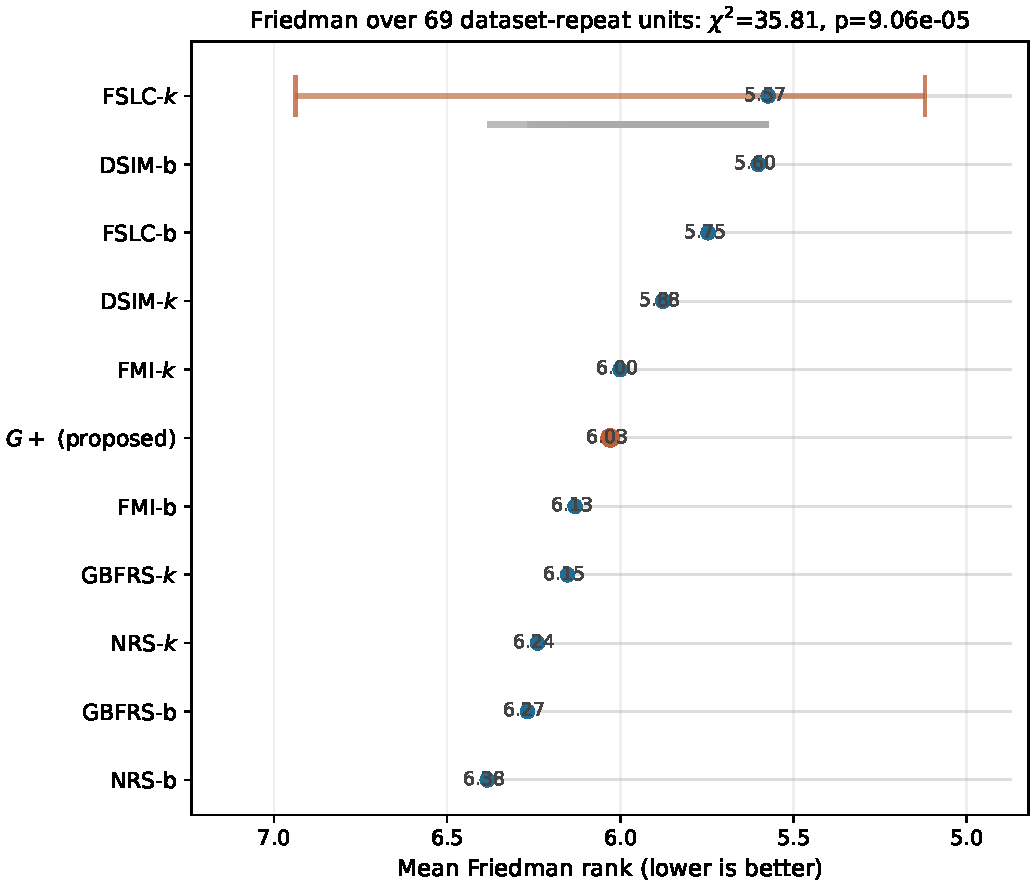
\includegraphics[width=\linewidth,height=.45\textheight,keepaspectratio]{paper_figures/expansion_cd.pdf}
	\caption{Mean Friedman ranks over the sixty-nine expansion dataset--repeat units (audit Brier; ties on guard-empty datasets receive average ranks), one row per method. The orange band is the Nemenyi critical difference (CD = 1.82) around $G+$; blue markers lie within it and are not statistically separated from $G+$.}
	\label{fig:expansion-cd}
\end{figure}
